\subsection{\labeltext[UC03 - Serviços]{UC3.1 - Requisitar livro}{uc:31}}
A imagem identificada como figura~\ref{fig:chap213} apresenta o diagrama de caso de uso \ref{uc:31} e tem como objetivo apresentar as interações entre os atores e o sistema.

\vspace*{5mm}

\begin{figure}[H]
	\centering
	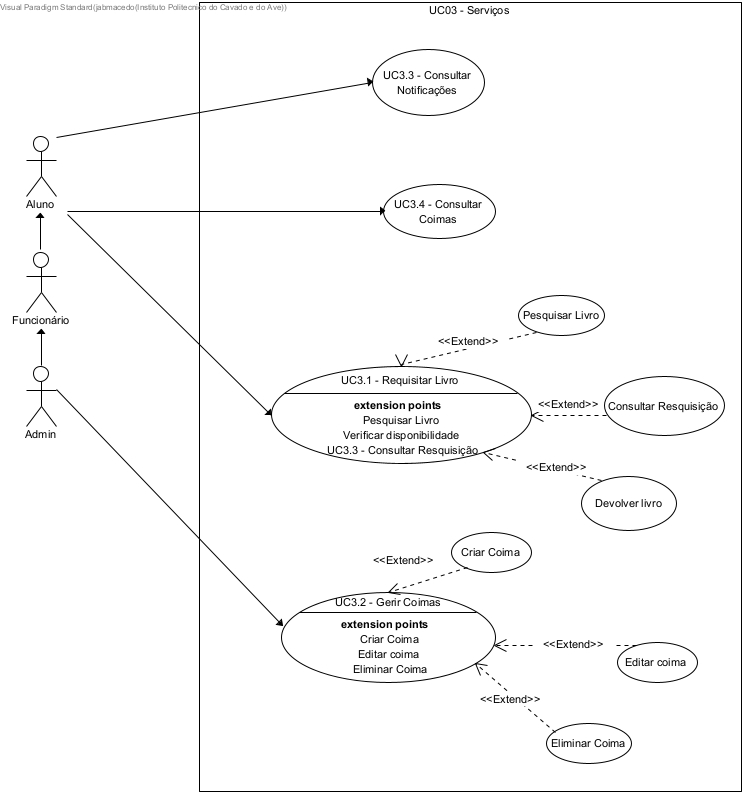
\includegraphics[width=1\linewidth]{./img/Diagramas\_UC/UC03.jpg}  % largura percentual 
	\caption{\ref{uc:31}}
	\label{fig:chap213}
\end{figure}

\newpage

\noindent \textbf{Descrição} \\
\textbf{ID:} UC3.1 \\  
\textbf{Nível de importância:} Alta \\
\textbf{Nome:} Requisitar livro \\
\textbf{Ator principal:} Aluno \\
\textbf{Atores secundários:} Funcionário, Administrador \\
\textbf{Breve descrição:} O aluno deverá conseguir requisitar livros. \\ 
\textbf{Ativador:} Intenção do aluno querer requisitar um livro.  \\
\textbf{Pré-condições:} Ter conta criada. \\
\textbf{Fluxo normal dos eventos:} \\
1. Abrir sistema.  \\
2. Autenticar-se no sistema. \\
3. Selecionar "Livros" \\
\textbf{Sub-fluxos:} \\ 
\indent A - Pesquisar livro\\
	\indent\indent A.1 - Este sub-fluxo inicia quando o utilizador deseja pesquisar um livro.\\
	\indent\indent A.2 - O sistema mostra a lista de livros.\\	
	\indent\indent A.3 - O utilizador insere o nome do livro a pesquisar.\\	
	\indent\indent A.4 - O utilizador carrega no botão "Pesquisar".\\	
	\indent\indent A.5 - O sistema mostra o resultado da pesquisa.\\	
	\indent\indent A.5 - O utilzador carrega no botão "Requisitar".\\
	\indent B - Devolver livro \\ 
	\indent\indent B.1 - Este sub-fluxo inicia quando o utilizador deseja devolver um livro.\\
	\indent\indent B.2 - O utilizador insere o livro a devolver e carrega "Devolver"\\
	\indent\indent B.3 - O sistema guarda os dados na base de dados e encaminha o utilizador para a página de requisição de livros.\\
	\indent C - Consultar requisção \\ 
	\indent\indent C.1 - Este sub-fluxo inicia quando o utilizador deseja consultar requisição de um livro.\\
	\indent\indent C.2 - O utilizador carrega no botão "Consultar resuisição".\\
	\indent\indent C.3 - O sistema devolve uma lista com as requisições do utilizador."\\
	\indent\indent C.4 - O utilizador carrega na requisição que deseja e é-lhe mostrada as informações sobre a requisição.\\
\textbf{Fluxos alternativos/excecionais:}  \\
	\indent A qualquer momento antes de submeter, o utilizador pode selecionar cancelar. A ação não é gravado e o caso de uso termina.\\

\newpage

\subsection{UC3.2 - Gerir coimas}
\vspace*{5mm}

\noindent \textbf{Descrição} \\
\textbf{ID:} UC3.2 \\  
\textbf{Nível de importância:} Alta \\
\textbf{Nome:} Gerir coimas \\
\textbf{Ator principal:} Administrador \\
\textbf{Atores secundários:} Funcionário \\
\textbf{Breve descrição:} O Administrador deverá conseguir criar, ediar e remover coimas do sistema. \\ 
\textbf{Ativador:} Necessidade do Administrador criar, editar ou remover uma coima.\\
\textbf{Pré-condições:} Ter nível de permissão de Administrador. \\
\textbf{Fluxo normal dos eventos:} \\
	\indent Caso de uso inicia quando o Administrador deseja gerir coimas. \\
	\indent De acordo com o tipo de operação que deseja efetuar é encaminhado para os seguintes sub-fluxo:\\
	\indent\indent A - Se o utilizador deseja criar/inserir coima, o sub-fluxo "Criar" é executado.\\
	\indent\indent B - Se o utilizador deseja editar uma coima, o sub-fluxo "Editar" é executado.\\
	\indent\indent C - Se o utilizador deseja remover uma coima, o sub-fluxo "Remover" é executado.\\
\textbf{Sub-fluxos:} \\
	\indent A - Criar coima\\
	\indent\indent A.1 - Este sub-fluxo inicia quando o utilizador deseja criar uma coima.\\
	\indent\indent A.2 - O utilizador insere os dados nos campos necessários.\\	
	\indent\indent A.3 - O utilizador com carrega no botão "Registar".\\	
	\indent\indent A.4 - O sistema guarda os dados na base de dados e encaminha para o menu gerir coimas.\\	
	\indent B - Editar coima \\ 
	\indent\indent B.1 - Este sub-fluxo inicia quando o utilizador deseja alterar informação de uma coima.\\
	\indent\indent B.2 - É apresentado ao utilizador a lista de coimas.\\
	\indent\indent B.3 - O utilizador edita os dados dos campos a editar.\\
	\indent\indent B.4 - O utilizador carrega no botão Atualizar.\\
	\indent\indent B.5 - O sistema guarda os dados na base de dados e encaminha para o menu gerir coimas.\\
	\indent C - Apagar coima  \\
	\indent\indent C.1 - Este sub-fluxo inicia quando o utilizador deseja apagar uma coima.\\
	\indent\indent C.2 - O sistema apresenta a lista de coimas.\\
	\indent\indent C.3 - O utilizador seleciona a coima que deseja apagar.\\
	\indent\indent C.4 - O sistema responde com uma mensagem "coima apagada com sucesso." e encaminha para o menu gerir coimas.\\
\textbf{Fluxos alternativos/excecionais:}  \\
	\indent A qualquer momento antes de submeter, o utilizador pode selecionar cancelar. A ação não é gravado e o caso de uso termina.\\
	\indent A - Criar coima\\
	\indent\indent A.5 - Se alguma informação estiver incorreta, o sistema pede ao utilizador para corrigir a informação.\\
	\indent B - Editar coima\\
	\indent\indent B.6 - Se alguma informação estiver incorreta, o sistema pede ao utilizador para corrigir a informação.\\

\newpage

\newpage

\subsection{UC3.3 - Consultar notificações}
\vspace*{5mm}

\noindent \textbf{Descrição} \\
\textbf{ID:} UC3.2 \\  
\textbf{Nível de importância:} Média \\
\textbf{Nome:} Consultar notificações \\
\textbf{Ator principal:} Aluno \\
\textbf{Atores secundários:} --------- \\
\textbf{Breve descrição:} O aluno deverá conseguir consultar as notificações que lhe são enderessadas. \\ 
\textbf{Ativador:} Necessidade do aluno querer consultar as notificações.\\
\textbf{Pré-condições:} Autenticar-se no sistema. \\
\textbf{Fluxo normal dos eventos:} \\
	\indent Caso de uso inicia quando o aluno deseja consultar as notificações. \\
	\indent O aluno clica em "Notificações".
	\indent O sistema devolve as notificações correspondentes.
\textbf{Sub-fluxos:} ---------\\
\textbf{Fluxos alternativos/excecionais:}  \\
	\indent A qualquer momento antes de submeter, o aluno pode selecionar cancelar. A ação não é gravado e o caso de uso termina.\\

	\subsection{UC3.4 - Consultar coimas}
\vspace*{5mm}

\noindent \textbf{Descrição} \\
\textbf{ID:} UC3.2 \\  
\textbf{Nível de importância:} Média \\
\textbf{Nome:} Consultar coimas \\
\textbf{Ator principal:} Aluno \\
\textbf{Atores secundários:} --------- \\
\textbf{Breve descrição:} O aluno deverá conseguir consultar as coimas que lhe são enderessadas. \\ 
\textbf{Ativador:} Necessidade do aluno querer consultar as coimas.\\
\textbf{Pré-condições:} Autenticar-se no sistema. \\
\textbf{Fluxo normal dos eventos:} \\
	\indent Caso de uso inicia quando o aluno deseja consultar as coimas. \\
	\indent O aluno clica em "Coimas".
	\indent O sistema devolve as coimas correspondentes.
\textbf{Sub-fluxos:} ---------\\
\textbf{Fluxos alternativos/excecionais:}  \\
	\indent A qualquer momento antes de submeter, o aluno pode selecionar cancelar. A ação não é gravado e o caso de uso termina.\\

\newpage